\documentclass[nooutcomes]{ximera}
%% handout
%% space
%% newpage
%% numbers
%% nooutcomes


\newcommand{\RR}{\mathbb R}
\renewcommand{\d}{\,d}
\newcommand{\dd}[2][]{\frac{d #1}{d #2}}
\renewcommand{\l}{\ell}
\newcommand{\ddx}{\frac{d}{dx}}
\newcommand{\dfn}{\textbf}
\newcommand{\eval}[1]{\bigg[ #1 \bigg]}

\usepackage{multicol}

\renewenvironment{freeResponse}{
\ifhandout\setbox0\vbox\bgroup\else
\begin{trivlist}\item[\hskip \labelsep\bfseries Solution:\hspace{2ex}]
\fi}
{\ifhandout\egroup\else
\end{trivlist}
\fi} %% we can turn off input when making a master document

\title{Section - 2.5:  Limits at Infinity (Solutions)}  

\begin{document}
\begin{abstract}		\end{abstract}
\maketitle

\section*{Warm up:}  
Match functions 1-6 with graphs A-F in the figure without using a graphing utility.
	\begin{enumerate}[label=\arabic*.]
	\item $f(x) = \frac{x}{x^2 + 1}$  
	\item $f(x) = \frac{x}{x^2 -1}$
	\item $f(x) = \frac{1}{x^2 -1}$
	\item $f(x) = \frac{x}{(x-1)^2}$
	\item $f(x) = \frac{1}{(x-1)^2}$
	\item $f(x) = \frac{x}{x+1}$
	\end{enumerate}
	
	\begin{image}
	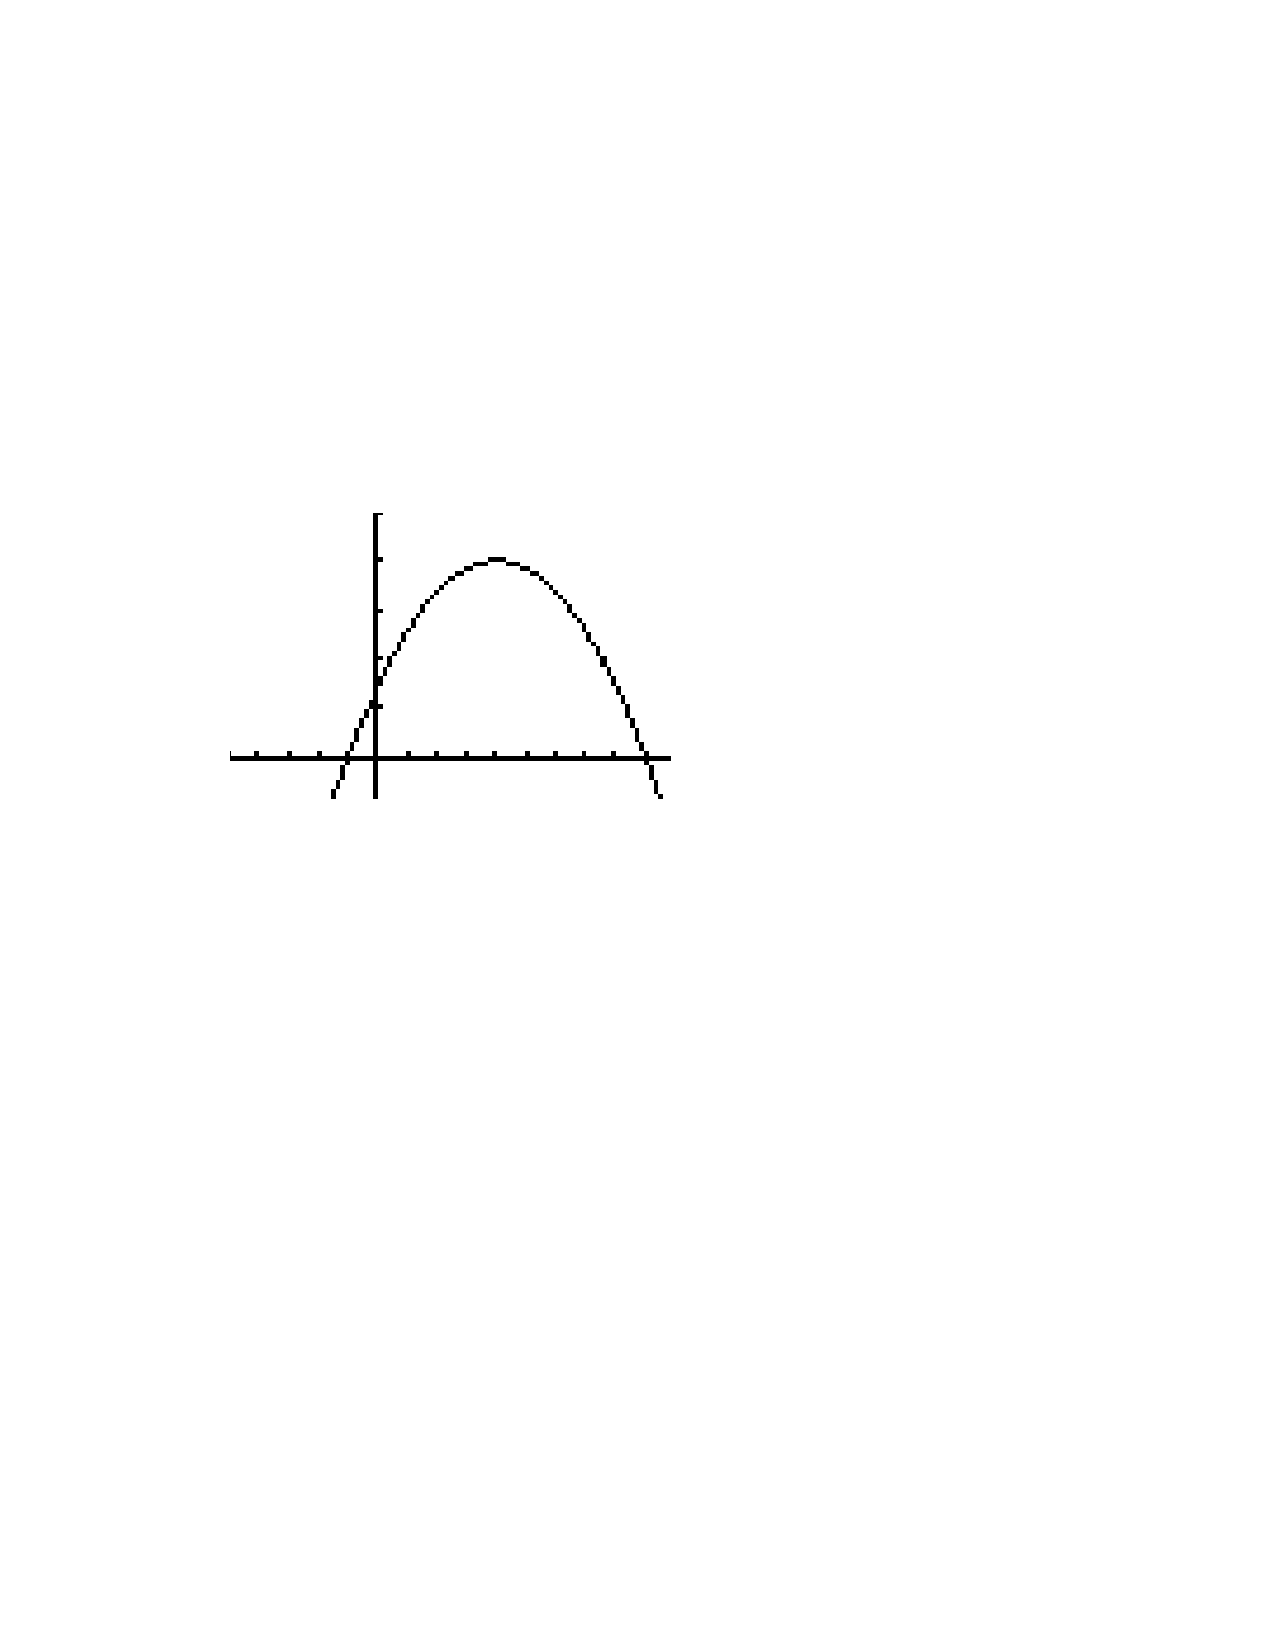
\includegraphics[trim= 250 360 300 185]{Figure1.pdf}
	\end{image}

	
		\begin{freeResponse} 
			\begin{enumerate}[label=\arabic*.]  
			\item  This is the only one without a vertical asymptote, (there is no value of $x$ for which $x^2 + 1$ equals 0).  So this one must be D.
			
			\item  $f(x)$ has a vertical asymptote at both $x=-1,1$ (found by solving $x^2 - 1 = 0$).  Since the degree of the numerator is one less than the degree of the denominator, there is a horizontal asymptote at $y=0$.  We then find that $f(0)=0$, so this one is C.
			
			\item  $f(x)$ has a vertical asymptote at both $x=-1,1$ (found by solving $x^2 - 1 = 0$).  $f(0) = -1$, so this one is F.  
			
			\item  $f(x)$ has a vertical asymptote at $x=1$ (found by solving $(x-1)^2 = 0$).  Since the degree of the numerator is one less than the degree of the denominator, there is a horizontal asymptote at $y=0$.  $f(0)=0$, and so this one is B.
			
			\item  $f(x)$ has a vertical asymptote at $x=1$ (found by solving $(x-1)^2 = 0$).  Since the degree of the numerator is less than the degree of the denominator, there is a horizontal asymptote at $y=0$.  $f(0)=1$, and so this one is A.
			
			\item  $f(x)$ has a vertical asymptote at $x=-1$ (found by solving $x+1=0$).  Since the degree of the denominator and numerator are the same, we find the horizontal asymptote by dividing the coefficients of the leading term to find $y=1$.   $f(0)=0$, and so this one is E.
	\end{enumerate}
		\end{freeResponse}
	
	
	
	



\section*{Group work:}

%problem 1
\begin{problem}
Find any vertical or horizontal asymptotes for the given function.  Be sure to tell where the function crosses its horizontal or vertical asymptote.  Also, when finding vertical asymptotes, be sure to say how the function approaches the asymptote on each side:

	\begin{enumerate}
	
	%part a
	\item  $f(x) = \frac{\sqrt{2x^2 + 1}}{3x-5}$
		
		\begin{freeResponse}
		To find the vertical asymptote, solve:
		
		$3x-5=0 \qquad \Longrightarrow \qquad 3x = 5 \qquad \Longrightarrow \qquad x = \frac{5}{3}.$
		
		$\lim_{x \to \frac{5}{3}^+} \frac{\sqrt{2x^2 + 1}}{3x-5} = \infty$ and $\lim_{x \to \frac{5}{3}^-} \frac{\sqrt{2x^2 + 1}}{3x-5} = - \infty$ since in both limits the numerator approaches $\frac{\sqrt{59}}{3}$, but the denominator of the first limit approaches $0$ from the right whereas the denominator of the second limit approaches $0$ from the left.
		
		To find the horizontal asymptotes:
		
		(as $x \to \infty$)  $\lim_{x \to \infty} \frac{\sqrt{2x^2 + 1}}{3x-5} 
		= \lim_{x \to \infty} \frac{\sqrt{2x^2 + 1}}{3x-5} \cdot \frac{\frac{1}{x}}{\frac{1}{x}} 
		= \lim_{x \to \infty} \frac{\frac{\sqrt{2x^2 + 1}}{x}}{\frac{3x-5}{x}} 
		= \lim_{x \to \infty}  \frac{\frac{\sqrt{2x^2 + 1}}{\sqrt{x^2}}}{3 - \frac{5}{x}} 
		= \lim_{x \to \infty}  \frac{\sqrt{\frac{2x^2 + 1}{x^2}}}{3 - \frac{5}{x}} 
		= \lim_{x \to \infty}  \frac{\sqrt{2 + \frac{1}{x^2}}}{3 - \frac{5}{x}} 
		= \frac{\sqrt{2+0}}{3-0} 
		= \frac{\sqrt{2}}{3} $
		
		(as $x \to -\infty$)  $\lim_{x \to -\infty} \frac{\sqrt{2x^2 + 1}}{3x-5} 
		= \lim_{x \to -\infty} \frac{\sqrt{2x^2 + 1}}{3x-5} \cdot \frac{\frac{1}{x}}{\frac{1}{x}} 
		= \lim_{x \to -\infty} \frac{\frac{\sqrt{2x^2 + 1}}{x}}{\frac{3x-5}{x}} 
		= \lim_{x \to -\infty}  \frac{\frac{\sqrt{2x^2 + 1}}{-\sqrt{x^2}}}{3 - \frac{5}{x}} 
		= \lim_{x \to -\infty}  -\frac{\sqrt{\frac{2x^2 + 1}{x^2}}}{3 - \frac{5}{x}} 
		= \lim_{x \to -\infty}  -\frac{\sqrt{2 + \frac{1}{x^2}}}{3 - \frac{5}{x}} 
		= -\frac{\sqrt{2+0}}{3-0} 
		= -\frac{\sqrt{2}}{3} $
		
		So there are horizontal asymptotes at $y = \pm \frac{\sqrt{2}}{3}$.  
		
		In order for the graph of $f(x)$ to cross $y = \frac{\sqrt{2}}{3}$, we must have that 
		$\frac{\sqrt{2x^2 + 1}}{3x-5} = \frac{\sqrt{2}}{3}
		\qquad \Longrightarrow \qquad 3 \sqrt{2x^2+1} = \sqrt{2}(3x-5)
		\qquad \Longrightarrow \qquad 9 (2x^2 + 1) = 2(9x^2 - 30x + 25)
		\qquad \Longrightarrow \qquad 18x^2 + 9 = 18x^2 - 60x + 50
		\qquad \Longrightarrow \qquad 60x = 41
		\qquad \Longrightarrow \qquad x = \frac{41}{60}$.
		
		We need to check this:  $f \left( \frac{41}{60} \right) = -\frac{\sqrt{2}}{3}$.  So the graph of $f(x)$ never crosses the line $y= \frac{\sqrt{2}}{3}$, but it crosses $y= -\frac{\sqrt{2}}{3}$ at the point $\left( \frac{41}{60}, - \frac{\sqrt{2}}{3} \right)$.  
		\end{freeResponse}
	
	
	
	%part b
	\item  $f(x) = \sqrt{x^2 + 8x + 1} - x$
	
		\begin{freeResponse}
		To find the vertical asymptotes of $f(x)$, we first need to find the domain of $f$.  This is where $x^2 + 8x + 1 > 0$.  $x^2 + 8x + 1 = 0$ when $x = -4 \pm \sqrt{15}$.   Using a sign chart, we determine that $x^2 + 8x + 1 > 0$ when $x < -4 - \sqrt{15}$ and $x > -4 + \sqrt{15}$.  Thus, the domain of $f(x)$ is $(-\infty, -4-\sqrt{15}) \cup (-4 + \sqrt{15}, \infty)$.  
		
		For any $a$ in $(-\infty, -4-\sqrt{15}) \cup (-4 + \sqrt{15}, \infty)$, $\lim_{x \to a} \sqrt{x^2 + 8x + 1} - x \neq \pm \infty$.  The same is true if $a = -4 \pm \sqrt{15}$.  So $f(x)$ has no vertical asymptotes.
		
		To find the horizontal asymptotes:
		
		(as $x \to \infty$)  $\lim_{x \to \infty} \sqrt{x^2 + 8x + 1} - x
		= \lim_{x \to \infty} \left( \sqrt{x^2 + 8x + 1} - x \right) \cdot \left( \frac{\sqrt{x^2 + 8x + 1} + x}{\sqrt{x^2 + 8x + 1} + x} \right) 
		=  \lim_{x \to \infty} \frac{x^2 + 8x + 1 - x^2}{\sqrt{x^2 + 8x + 1} + x} 
		= \lim_{x \to \infty} \frac{x \left( 8 + \frac{1}{x} \right)}{x \left( \sqrt{1 + \frac{8}{x} + \frac{1}{x^2}} + 1 \right)}
		= \lim_{x \to \infty} \frac{8 + \frac{1}{x}}{\sqrt{1 + \frac{8}{x} + \frac{1}{x^2}} + 1} 
		= \frac{8 + 0}{\sqrt{1 + 0 + 0} + 1}
		= \frac{8}{2} = 4.$
		
		(as $x \to -\infty$)  $\lim_{x \to -\infty} \sqrt{x^2 + 8x + 1} - x
		= \lim_{x \to -\infty} \left( \sqrt{x^2 + 8x + 1} - x \right) \cdot \left( \frac{\sqrt{x^2 + 8x + 1} + x}{\sqrt{x^2 + 8x + 1} + x} \right) 
		=  \lim_{x \to -\infty} \frac{x^2 + 8x + 1 - x^2}{\sqrt{x^2 + 8x + 1} + x} 
		= \lim_{x \to -\infty} \frac{x \left( 8 + \frac{1}{x} \right)}{-x \left( \sqrt{1 + \frac{8}{x} + \frac{1}{x^2}} + 1 \right)}
		= \lim_{x \to -\infty} - \frac{8 + \frac{1}{x}}{\sqrt{1 + \frac{8}{x} + \frac{1}{x^2}} + 1} 
		= -\frac{8 + 0}{\sqrt{1 + 0 + 0} + 1}
		= -\frac{8}{2} = -4.$
		
		So there are horizontal asymptotes at $y = \pm 4$. 
		
		In order for the graph of $f(x)$ to cross $y = \pm 4$, we must have that 
		$ \sqrt{x^2 + 8x + 1} - x = \pm 4
		\qquad \Longrightarrow \qquad \sqrt{x^2 + 8x + 1} = x \pm 4
		\qquad \Longrightarrow \qquad x^2 + 8x + 1 = x^2 \pm 8x + 16
		\qquad \Longrightarrow \qquad 8x = \pm 8x + 15.$
		
		So if $y = 4$, then the above equation becomes $0 = 15$ and thus there are no solutions.
		
		If $y=-4$, then the above equation becomes $16x = 15$ and thus $x = \frac{15}{16}$.
		
		Therefore, the graph of $f(x)$ never crosses the horizontal asymptote $y = 4$, and it crosses $y = -4$ at the point $\left( \frac{15}{16}, -4 \right)$.  
		
		\end{freeResponse}
	
	\end{enumerate}
	
\end{problem}
			
			
			
			


%problem 2
\begin{problem}	
Find any vertical, horizontal, or slant asymptotes for the function $f(x) = \frac{x^2 + 7x + 11}{x-3}$.  Be sure to tell where the function crosses its horizontal or vertical asymptotes.  Also, when finding vertical asymptotes, be sure to say how the function approaches the asymptote on each side.

		\begin{freeResponse}
		
		To find the vertical asymptote, we solve $x - 3 = 0$, and so $x = 3$.  
		
		$\lim_{x \to 3^-}  \frac{x^2 + 7x + 11}{x-3} = -\infty$ and $\lim_{x \to 3^+}  \frac{x^2 + 7x + 11}{x-3} = \infty$ since, in both cases the numerator approaches $41$, but in the first limit the denominator approaches $0$ from the left whereas in the second limit the denominator approaches $0$ from the right.
		
		\dfn{Because the degree of the numerator is one higher than the degree of the denominator, this function has a slant asymptote.}  Performing long division, we see that $\frac{x^2 + 7x + 11}{x-3} = x + 10 - \frac{41}{x-3}$.  Thus, $y = x+10$ is a slant asymptote for $f(x)$.  $f(x)$ has no horizontal asymptotes.
		
		\end{freeResponse}
\end{problem}







%problem 3
\begin{problem}	
Sketch the graph of a function with all of the following properties:

	$\lim_{x \to -2^-} f(x) = \infty, 
	f(-2) = 7, 
	f(1) = 2, 
	\lim_{x \to \infty} f(x) = 3, 
	\lim_{x \to -\infty} f(x) = -\infty,$
\newline 
	$\lim_{x \to 5} f(x) = \infty, 
	\lim_{x \to 9} f(x) = 3,  
	f(9) = 1,  
	\lim_{x \to -3^-} f(x) = \infty,  
	\lim_{x \to -3^+} f(x) = -\infty,$
\newline  
	$f(4) \text{ is undefined, }
	f(x) = 3 \text{ for } x>9  $
	
		\begin{freeResponse}
			\begin{image}
			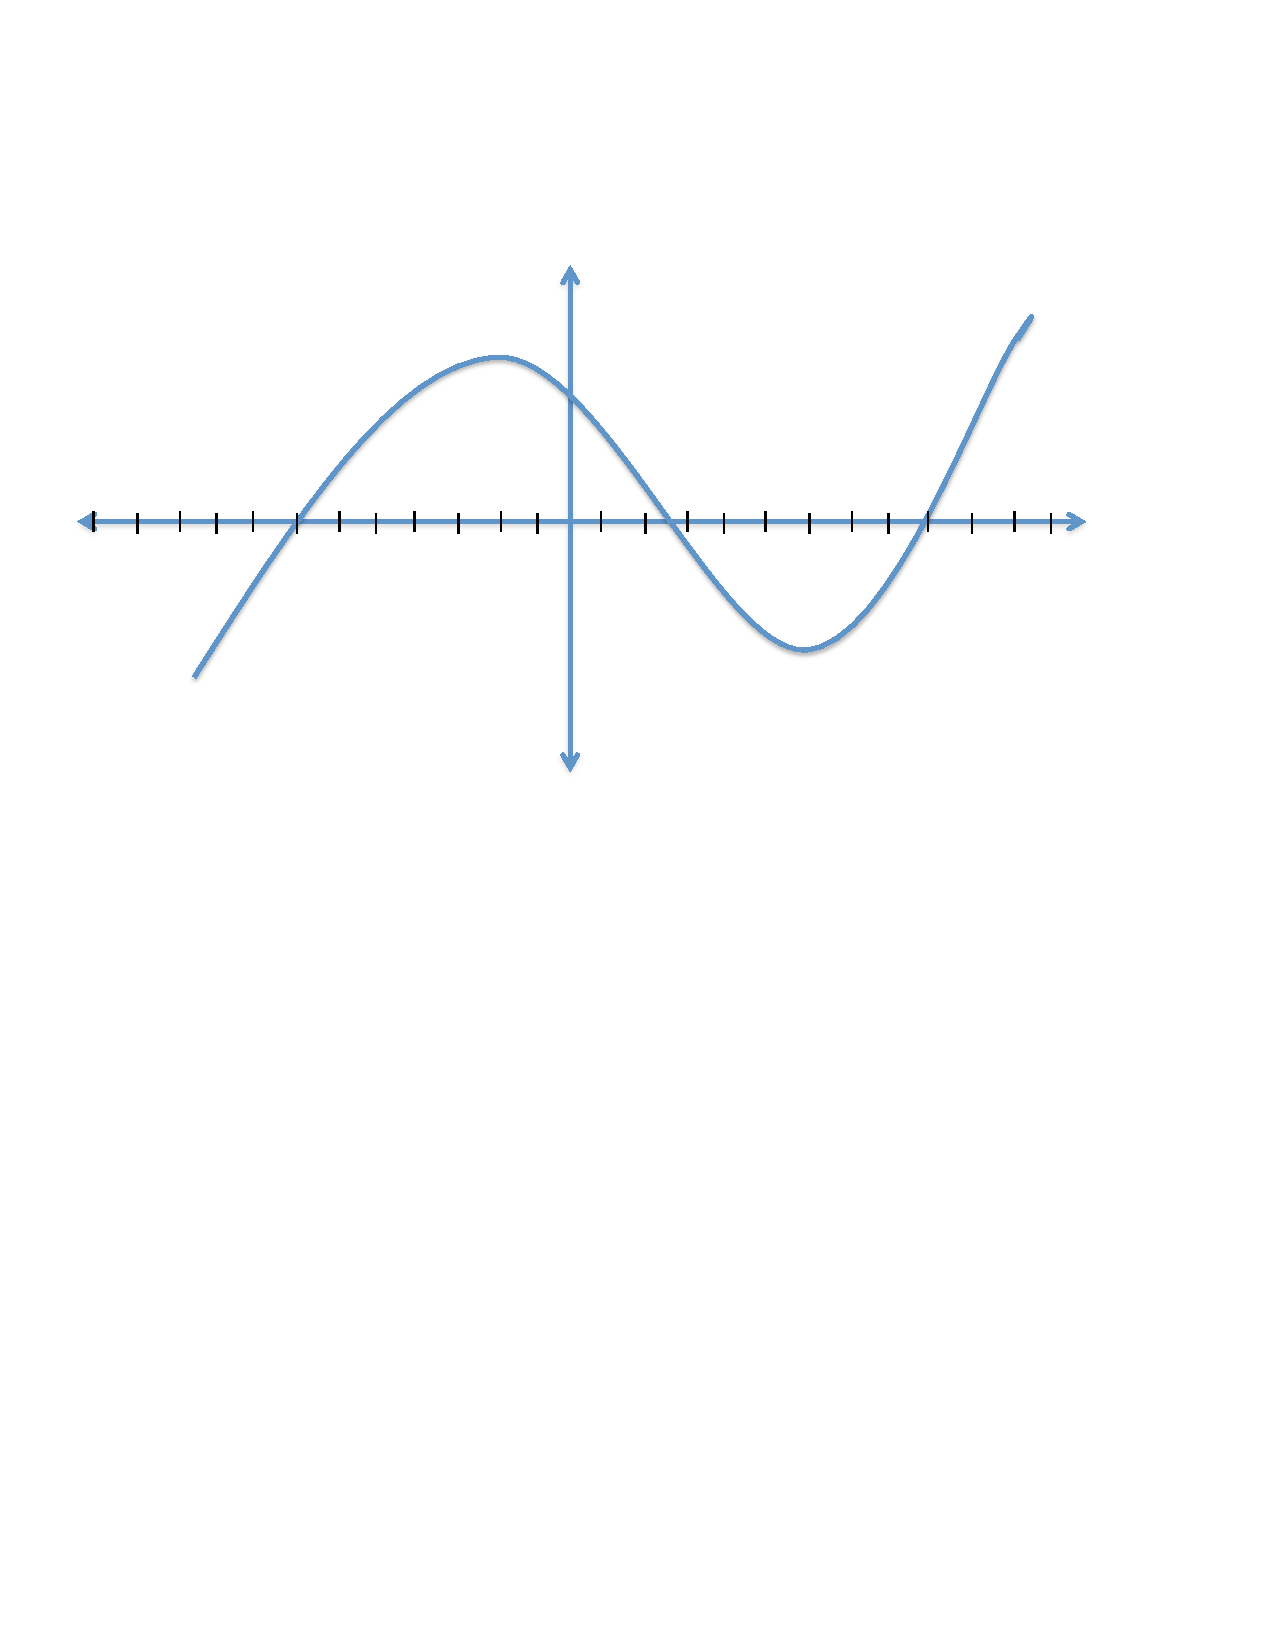
\includegraphics[trim= 100 360 300 175]{Figure2.pdf}
			\end{image}
		\end{freeResponse}
\end{problem}



























\end{document} 


















